\chapter{Uso de GitHub para obtener y modificar el código fuente de la librería Materia}\label{chap:github}

Para mayor información sobre la participación en proyectos de GitHub, se recomienda la lectura de las guias:

\begin{itemize}\itemsep0ex
	\item Hola Mundo en GitHub, \url{https://guides.github.com/activities/hello-world/}
	\item Copias personales `Forking', \url{https://guides.github.com/activities/forking/}
	\item Seguimiento de errores y mejoras, \url{https://guides.github.com/features/issues/}
	\item Contribuyendo a proyectos Open-Source, \url{https://guides.github.com/activities/contributing-to-open-source/}
\end{itemize}

Para mayor información sobre Git se recomienda leer la documentación de la página oficial:
\begin{itemize}\itemsep0ex
	\item \url{http://git-scm.com/}
\end{itemize}

	A continuación se listan brevemente los pasos necesarios para obtener y contribuir a la bliblioteca de clases Materia, es necesario tener una cuenta en GitHub y tener instalado \href{http://git-scm.com/}{Git} en la computadora.

	\begin{enumerate}\itemsep0ex
		\item Encuentra algo en qué trabajar. Ya sea que encuentres un error en la biblioteca, quieras realizar una mejora o crear una nueva función primero debes estar seguro de lo que quieres hacer. 

		\item Archiva el asunto. Para evitar que dos personas trabajen en el mismo error, o intenten crear funciones semejantes es necesario llevar un registro de lo que se esta realizando en la biblioteca, para ello existe la sección `issues' en la página de GitHub de la biblioteca Materia \url{https://github.com/HugoRedon/Materia}. Ver la figura \ref{fig:issuesMateria}. Para mas información sobre como archivar asuntos en GitHub referirse a la guía de ayuda \url{https://guides.github.com/features/issues/}.

		\begin{figure}[!h]
			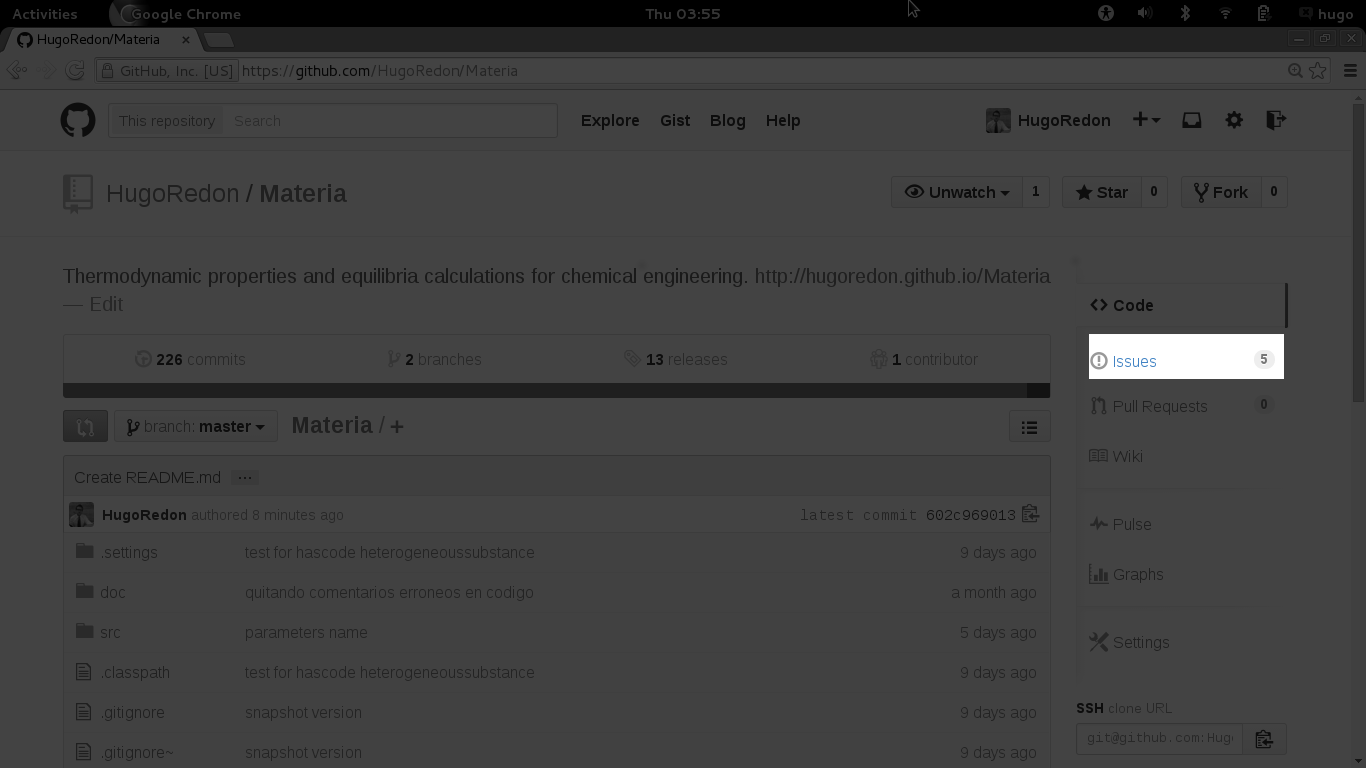
\includegraphics[scale=0.3]{materiaIssues.png}
			\caption{Página de GitHub de la biblioteca Materia, la sección resaltada permite archivar asuntos de error o mejoras en la biblioteca.}
			\label{fig:issuesMateria}
		\end{figure}

		\item Crea una copia personal de la biblioteca en tu cuenta de GitHub `Fork'. Para realizar una copia solo debes dirigirte a la página de GitHub del proyecto \href{https://github.com/HugoRedon/Materia}{Materia} y dar click en el boton `Fork', ver la figura \ref{fig:forkMateria}.

		\begin{figure}[!h]
			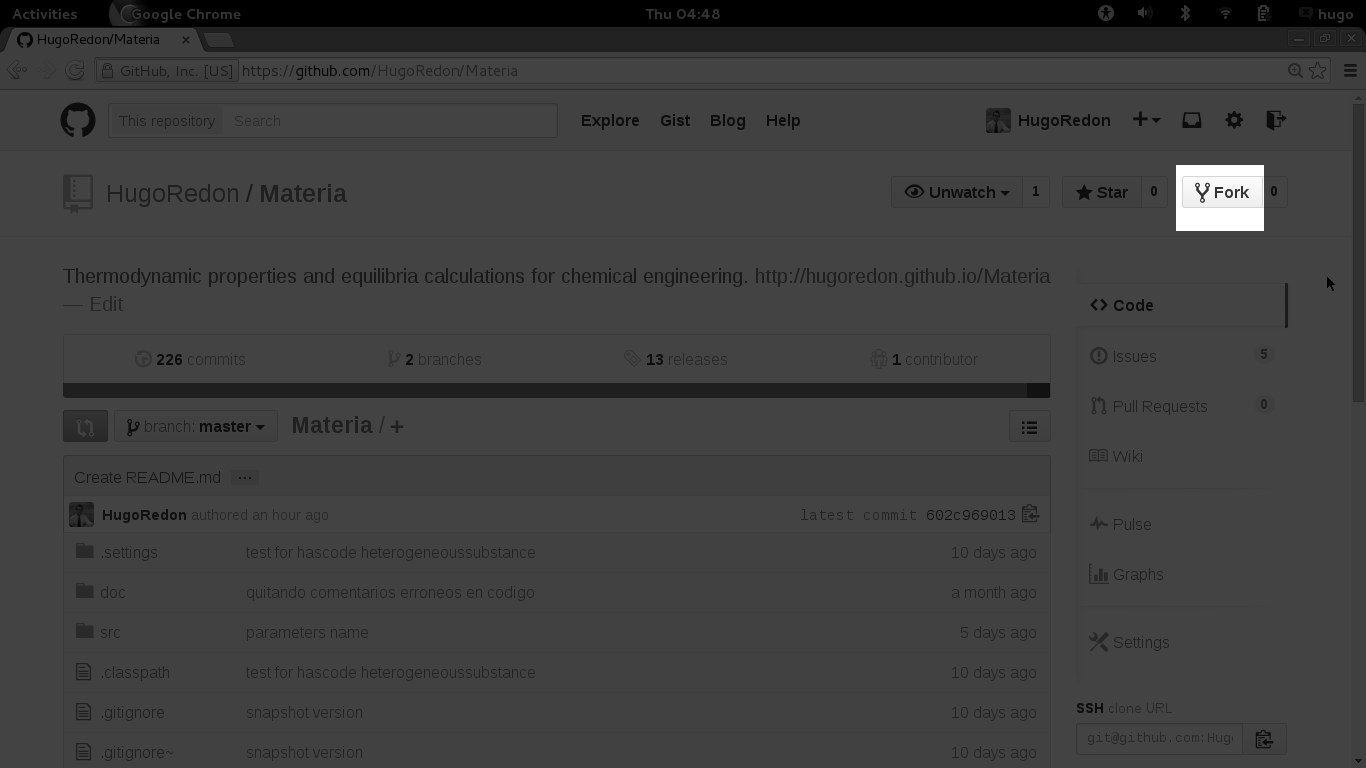
\includegraphics[scale=0.3]{forkMateria.png}
			\caption{Para realizar una copia personal de la biblioteca Materia solo se debe dar click en el boton `Fork'}
			\label{fig:forkMateria}
		\end{figure}

		\item Clona tu copia personal de la biblioteca Materia en tu computadora. 
			\begin{itemize}\itemsep0ex
				\item En github navega a tu copia personal del proyecto Materia
				\item En la barra derecha de la página, da click en el boton 
\includegraphics{clonebutton.png} para copiar la url del repositorio.
				\begin{figure}[!h]
					\centering
					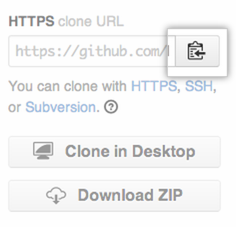
\includegraphics[scale=0.5]{cloneArea.png}.
				\end{figure}
				\item Abre una terminal (para usuarios de Mac y Linux) o linea de comando (usuarios de Windows).
				\item Escribe el comando  `git clone' y después pega la url del paso 2. El resultado debe ser algo semejante al código \ref{lst:cloneCommand}

\begin{lstlisting}[label={lst:cloneCommand},caption={Commando para clonar el repositorio de GitHub},language=bash]
	$ git clone https://github.com/<Nombre de usuario>/Materia
\end{lstlisting}

			\end{itemize}

		\item Crear la rama donde se realizarán los cambios. Para trabajar de forma segura se debe crear una rama donde se desarrollen las nuevas funciones o la corrección a la librería Materia. Esto se logra con el commando \ref{lst:newBranch}. El nombre de la nueva rama debe ser consistente con la tarea a realizar.
		\begin{lstlisting}[label={lst:newBranch},caption={Commando para crear una nueva rama en el repositorio.},language=bash]
			$ git checkout -b <nombre de la nueva rama>
		\end{lstlisting}
	\end{enumerate}


